% Created 2013-12-20 金 04:52
\documentclass[12pt]{jsarticle}
\usepackage[dvipdfmx]{graphicx}
\usepackage{comment}
%\usepackage{setspace}
%%\date{\today}
%\title{}
\textheight = 25truecm
\textwidth = 18truecm
\topmargin = -1.5truecm
\oddsidemargin = -1truecm
\evensidemargin = -1truecm
\marginparwidth = -1truecm
\def\theenumii{\Alph{enumii}}
\def\theenumiii{\alph{enumiii}}
\def\labelenumi{(\theenumi)}
\def\labelenumiii{(\theenumiii)}
%\setstretch{0.9}
\begin{document}

%\maketitle
%\tableofcontents

\begin{center}
%%%%%%%%%%%%%%%%%%%%%%%%%%%%%%%%%%%%%%%
%%%タイトル                         %%%
%%%%%%%%%%%%%%%%%%%%%%%%%%%%%%%%%%%%%%%
{\LARGE 「SMPを利用したPrimary/Backupモデルによるリプレイ環境の構築」の要約}
\end{center}

\begin{flushright}
  2014/6/18\\
  藤田将輝
\end{flushright}
%%%%%%%%%%%%%%%%%%1章%%%%%%%%%%%%%%%%%%%
\section{はじめに}
Primary/Backupを用いたOSのデバッグ方法を理解するため,情報処理学会研究報告である
「SMPを利用したPrimary/Backupモデルによるリプレイ環境の構築」
\cite{bib1}を読解した.
本資料ではこの論文の要約を示す.


\section{目的}
OSの開発時やシステム運用時にカーネルパニックによる障害が発生することがある.
この原因を特定するには過去の状態を推定する必要がある.
デバッグ時に,利用できる情報はカーネルパニック後の
ものに限られる.
このため,原因の特定が容易ではない.
特に,再現性の低いバグに起因する場合や,ダンプデータが破壊されている場合には原因の特定がさらに困難なものとなる.
そこで,本研究では,仮想マシンモニタを応用し,カーネルパニック後の状態だけでなく,カーネルパニック前の
状態も再現することで,効率的なデバッグ環境を提供する.
本研究ではマルチプロセッサのSMP環境を活用し,Primary/Backupモデルにより,2つのOSを時間差を設けて実行する方法を提案する.
なお,SMPとはSymmetric Multiprocessing(対称型マルチプロセッシング)のことである.
2つのOSをそれぞれPrimaryとBackupに割り当て,それらを時間差を設けて実行することで,Primaryのカーネルパニック時にBackup側で
カーネルパニックが起きる前の状態を再現できる.



\section{システム概要}
\subsection{概要}
本研究のシステム概要図を図1に示し,以下で説明する.
SMP上でPrimaryとBackupの2つのVMを実行する.
Core0をPrimaryに割り当て,Core1をBackupに割り当てている.
そして,Primary/Backup間でロギングとリプレイを実現することにより,BackupでPrimaryの過去の状態を再現する.
ここで,ロギングとは,OSの実行を通常に行い,ログの取得と保存を行うことである.
また,リプレイとはログの読出しとOSの再現実行をすることである.
ここでのログとはOSの動作を再現するために必要な情報である.
本稿ではこのログを実行履歴と呼ぶ.
デバッグ時には再現した状態を利用する.






\begin{figure}[t]
\begin{center}
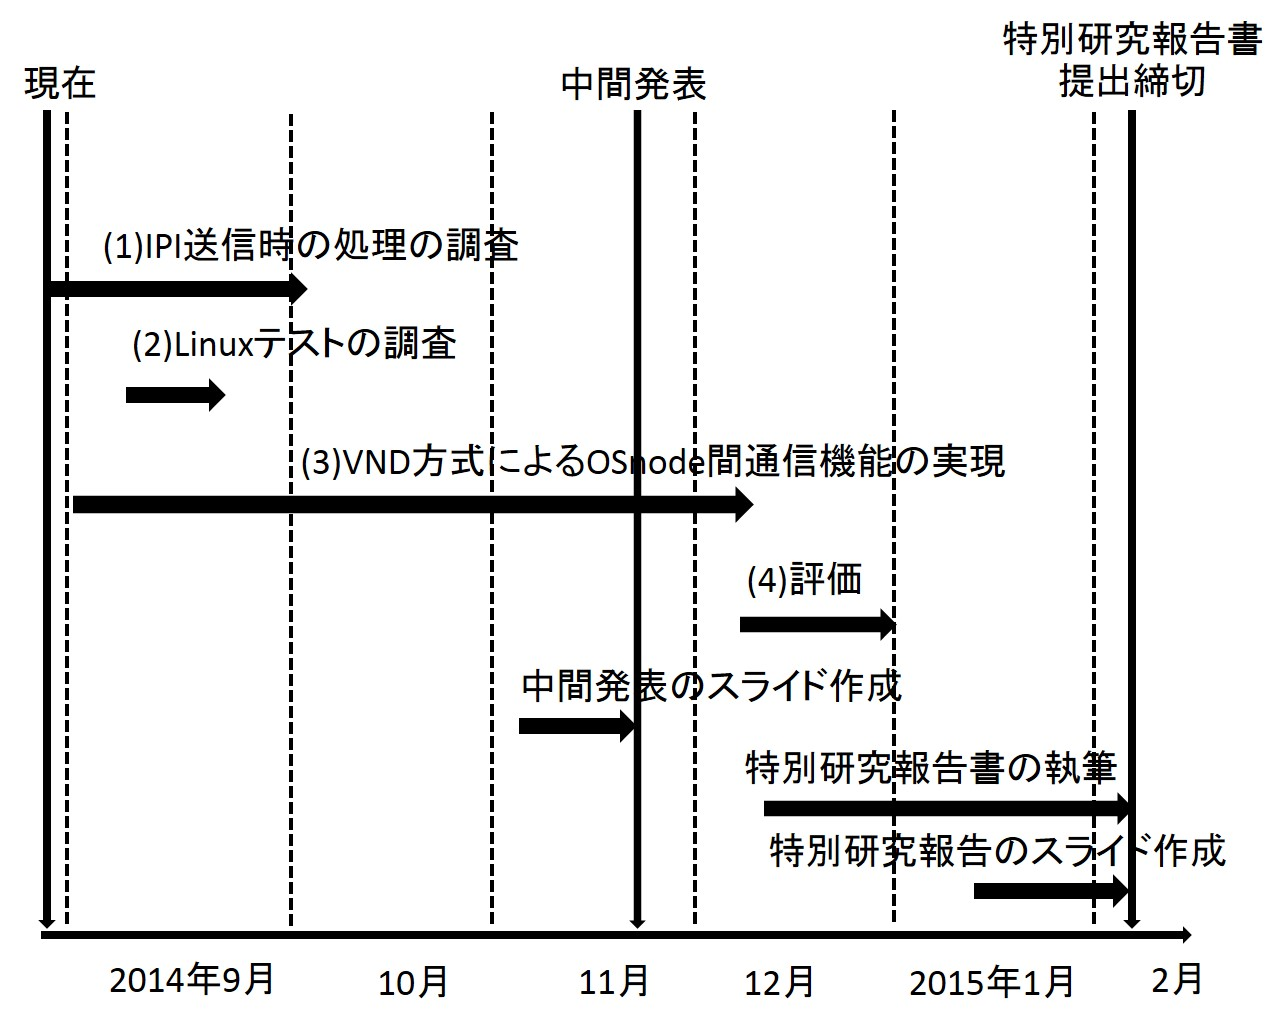
\includegraphics[height=5.5cm]{./fig1.jpg}          
\caption{システム概要図}
\label{fig:up}
\end{center}
\end{figure}





\subsection{機能}
本システムは,PrimaryでゲストOSを起動し,BackupはPrimaryよりも遅れて実行を開始する.
このとき,2つのOSは完全に同一な挙動を示すようにする.
その結果,Primaryのカーネルが不具合を起こし,停止した時点において,Backup側は不具合を発生する前の状態
となる.
デバッグではこの時点のBackup側のOSを利用する.
また,このリプレイ操作は何度でも繰り返して実行できる.

\subsection{要求}
3.2で述べた機能を実現するためには,PrimaryとBackup間で仮想マシンが同一の状態を保っていなければならない.
2つの仮想マシンを同一の状態に保つには以下の要件を満たす必要がある.
\begin{enumerate}
\item イベントを同一のタイミングで処理し,同一の結果を得ること.
\item 命令列を同一の順序で処理し,同一の結果を得ること.
\end{enumerate}
2つの仮想マシンを同一の状態に保つために,Primary からBackupに命令と割り込みのタイミング,実行結果を
通知する.

\subsection{実現方法}
本研究では3.3の要求を踏まえて,仮想マシンモニタを利用する.
Primaryではロギングを行い,Backupではリプレイを行う.
また,PrimaryとBackup間で非同期的なイベントのタイミングと命令に関する情報を転送する必要がある.
このため,PrimaryとBackup間を共有メモリを用いて結合し,情報をPrimaryからBackupへ通知する.


\section{ロギング\&リプレイ}
\subsection{実行履歴の種類}
Primaryでの動作をBackupで再現するためには,PrimaryとBackup間で同一の状態を保つことが求められる.
このためには,2つの仮想マシンにおいて割り込みなどの非同期的なイベントを同一のタイミングで処理し同一の結果を得ること,
また命令列を同一順序で処理し同一の結果を得ることが必要である.
これらを実現するには,PrimaryからBackupに実行履歴を通知する必要がある.
具体的には
非同期的なイベントの種類と起きたタイミングとその内容,また,結果が外部要因に影響を受ける命令と,その結果
を実行履歴をして転送することが求められる.
実行履歴として,本研究では以下の情報のうちイベントごとに必要なものを実行履歴として保存する.
\begin{enumerate}
\item イベントの種類\\
イベントの種類を識別するために必要である.具体的には,割り込みなのか命令なのか,割り込みであれば
どの種類の割り込みなのか,命令であればどの種類の命令なのか,といった点を識別する値を保存する.
\item イベントの発生した命令アドレス\\
Backupに,Primaryと同一の命令アドレスでイベントの通知や結果の適用を行うために必要である.
\item 命令の実行結果\\
Primaryが非決定的な命令を実行した際に得られた結果を保存し,Backupで同一の命令が実行されたときに保存された結果の値を返すために必要である.
\item ECX\\
ECXをカウンタとして利用する命令を使用する際に,Primaryと同一のタイミングでBackupにイベントを通知するために必要である.
ECXとはx86が提供するカウンタレジスタである.
\item 分岐回数\\
命令のタイミングを特定するために必要である.
分岐命令を経由すると同一アドレスを複数回通過することになり,命令アドレスだけでは同一のタイミングを特定することができない.
そこで,分岐命令の回数を保存しておき,分岐命令の回数と命令アドレスにより同一のタイミングを特定する.
\end{enumerate}
\subsection{実行履歴の取得の流れ}
実行履歴の取得の流れを以下に示す.
\begin{enumerate}
\item Primaryは,非同期的にイベントが発生した際に,これを契機としてゲストOSから仮想マシンモニタに実行を遷移する.
\item 仮想マシンモニタが実行履歴を作成し,共有メモリにこれを格納する.
\item Backupの仮想マシンモニタでは,実行履歴を共有メモリから読み出し,ゲストOSに適切に通知する.
このとき,PrimaryとBackupとでイベント処理後の仮想マシン状態を同一のものにするため,
イベントはPrimaryで起きたものと同一のタイミングで同一の内容を通知する.
\end{enumerate}
\subsection{実現方法}
4.2で述べた処理の流れをを実現する方法として,分岐回数をカウントすることによりタイミングを求める方法をとる.
これには,IA-32アーキテクチャのPerformance Monitoring Counter(PMC)を利用する.
PMCは様々なハードウェアイベントを計測するために利用できるカウンタ群であり,複数のハードウェアイベントを同時に計測することができる.
本手法における実行の流れは以下のようになる.
\begin{enumerate}
\item PMCを設定し,分岐回数のカウントを開始する.
\item イベント発生時に分岐回数を含む実行履歴を取得し,共有メモリに格納する.
\item (1)に戻って処理を継続する.
\end{enumerate}
\subsection{実行履歴の転送}
Primary側で実行履歴を取得し,Backup側へと転送するために,前述のとおり共有メモリを利用する.
このため,物理メモリ上にPrimaryとBackupの両方からアクセスできる物理アドレス空間を確保する.
\subsection{実行履歴の再現}
Backupでは,共有メモリから実行履歴を読出し,ゲストOSに通知することにより仮想マシンの状態を
Primaryと同一の状態に保つ.非同期的なイベントについては以下のように処理する.なお,以下の操作はすべてBackupが行う.
\begin{enumerate}
\item 実行履歴を共有メモリから取得する.
\item 実行履歴の命令アドレスをもとに,その命令アドレスまで実行する.
\item 分岐回数とECXを比較する.
\begin{enumerate}
\item 一致すれば次に進む.
\item 一致しなければ(2)に戻り繰り返す.
\end{enumerate}
\item ゲストOSにイベントを通知する.
\item (1)に戻って処理を継続する.
\end{enumerate}
また,非決定的な命令については,当該命令を実行時に実際に命令を実行して結果を得るのではなく,実行履歴から得た結果を
ゲストOSに返すことで再現する.
\section{まとめ}
本稿ではカーネルデバッグの支援方法として,ロギング\&リプレイをSMPを活用して実現する手法を提案した.これは,SMPの各プロセッサ
をPrimaryとBackupに割り当てる方法であり,仮想マシンモニタにより実現する.BackupをPrimaryに対して時間差を設けて実行することで,
Primaryの過去の状態をBackupで再現できる.
\section{おわりに}
本資料では「SMPを利用したPrimary/Backupモデルによるリプレイ環境の構築」の要約を示した.
PrimaryとBackupを同一の状態にするために,Primaryで発生した非同期処理のタイミングや,非決定的な命令結果を
共有メモリに保存し,Backupに通知する仕組みを理解した.
山本凌平の特別研究報告にある,NICドライバの割り込み処理を対象としたデバッグ支援環境にも共有メモリが
使用されていたため,共有メモリを使った情報の受け渡しが大変参考になった.

\begin{thebibliography}{9}
\bibitem{bib1} 川崎仁,追川修一:SMP を利用したPrimary/Backup モデルによるリプレイ環境の構
築,情報処理学会研究報告,Vol.2010-OS-113,No.12,pp.1-8(2010).
\end{thebibliography}

\end{document}
